% !TEX TS-program = pdflatex
% !TEX encoding = UTF-8 Unicode

% TeX-M (r1.0)
% For my math classes at UT Austin
% Notes template created by Abdon Morales for the College of Natural Science
% and for the Department of Mathematics and Computer Science
% (c) 2019 - 2024 Abdon Morales and the University of Texas at Austin
% This is a notes template for a LaTeX document using the "article" class for Mathematics (Calculus)
% at the University of Texas at Austin.

% Last change made: Jan 15, 2024 8:41 PM CST

% See "book", "report", "letter" for other types of document.

\documentclass[11pt]{article} % use larger type; default would be 10pt

% Start of Article customization options and addons (for more help and information reference to Overleaf's guides and docs on Latex.
\usepackage[utf8]{inputenc} % set input encoding (not needed with XeLaTeX)

%%% Examples of Article customizations
% These packages are optional, depending whether you want the features they provide.
% See the LaTeX Companion or other references for full information.

%%% PAGE DIMENSIONS
\usepackage{geometry} % to change the page dimensions
\geometry{letterpaper} % or letterpaper (US) or a5paper or....
% \geometry{margin=2in} % for example, change the margins to 2 inches all round
% \geometry{landscape} % set up the page for landscape
%   read geometry.pdf for detailed page layout information

\usepackage{graphicx} % support the \includegraphics command and options

% \usepackage[parfill]{parskip} % Activate to begin paragraphs with an empty line rather than an indent

%%% PACKAGES
\usepackage{booktabs} % for much better looking tables
\usepackage{array} % for better arrays (eg matrices) in maths
\usepackage{paralist} % very flexible & customisable lists (eg. enumerate/itemize, etc.)
\usepackage{verbatim} % adds environment for commenting out blocks of text & for better verbatim
\usepackage{subfig} % make it possible to include more than one captioned figure/table in a single float
\usepackage{exercise}
% Math tools
\usepackage{mathtools}
\usepackage{amsmath}
\usepackage{tikz} % For charts, mathematical graphs, and etc
\usepackage{tcolorbox}
%% Equal symbol for L'Hospital Rule
\newcommand\LR{\stackrel{\mathclap{\normalfont\mbox{L.R}}}{=}}
% These packages are all incorporated in the memoir class to one degree or another...

%%% HEADERS & FOOTERS
\usepackage{fancyhdr} % This should be set AFTER setting up the page geometry
\pagestyle{fancy} % options: empty , plain , fancy
\renewcommand{\headrulewidth}{0pt} % customise the layout...
\lhead{}\chead{}\rhead{}
\lfoot{}\cfoot{\thepage}\rfoot{}

%%% SECTION TITLE APPEARANCE
\usepackage{sectsty}
\allsectionsfont{\sffamily\mdseries\upshape} % (See the fntguide.pdf for font help)
% (This matches ConTeXt defaults)

%%% ToC (table of contents) APPEARANCE
\usepackage[nottoc,notlof,notlot]{tocbibind} % Put the bibliography in the ToC
\usepackage[titles,subfigure]{tocloft} % Alter the style of the Table of Contents
\renewcommand{\cftsecfont}{\rmfamily\mdseries\upshape}
\renewcommand{\cftsecpagefont}{\rmfamily\mdseries\upshape} % No bold!
%%% END Article customizations

%%% The "real" document content comes below...

\title{Economic Growth and the Wealth of Nations}
\author{Abdon Morales \\ The University of Texas at Austin \\ ECO 304L \\ Wayne Geerling}
\date{\today \\ Chapter 11 : Week 5}
%\date{} % Activate to display a given date or no date (if empty),
         % otherwise the current date is printed 

\begin{document}
\maketitle
\subsection*{There's more to prosperity than natural resources}

Many people believe that natural resources, such as trees, oil, and farmland, are the primary sources of economic growth. They believe that nations like the United States and Australia are prosperous because these nations have vast natural resources to use in the production of goods and services. A variation on this idea emphasizes geography: nations with the best shipping locations and mildest climates have more prosperous economies.

Striving for economic growth is not only about accumulating more wealth. Yes, economic growth brings smartphones and Jet Skis, but it's much more important than that; economic growth offers the potential for more women and infants to survive childbirth, more people to have access to clean water and better sanitation, and more people to live healthier, longer, and more educated lives.

In this chapter, we begin by looking at the implications of economic growth for human welfare; we then consider the impact of an economy's resources and technology on economic growth. Finally, we discuss the key elements an economy needs in order to grow.
\begin{tcolorbox}[width=\textwidth,colback={white},title={Big Questions},colbacktitle=yellow,coltitle=blue]
\begin{itemize}
\item \textbf{Why does economic growth matter?}
	\subitem - Economic growth affects human welfare in meaningful ways.
	\subitem - Historical data show that sustained economic growth is a relatively modern phenomenon.
	\subitem - Relatively small but consistent growth rates are an effective path of poverty.
	
\item \textbf{How do resources and technology contribute to economic growth?}
	\subitem - Natural Resources, physical capital, and human capital all contribute to economic growth.
	\subitem - Technological advancement, which leads to the production of more output per unit of input, also sustains economic growth.
	
\item \textbf{What institutions foster economic growth?}
	\subitem - Private property rights secure ownership of what an individual produces, creating incentives for increased output.
	\subitem - Political stability and the rule of law allow people to make production decisions without concern for corrupt government.
	\subitem - Competitive and open markets allow everyone to benefit from global productivity.
	\subitem - Efficient taxes are high enough to support effective government, but low enough to provide positive incentives for production.
	\subitem - Stable money and prices allow people to make long-term production decisions with minimal risk.
	
\item \textbf{How are some economists testing new ideas?}

	\subitem - Fieldwork using randomized controlled trials (RCTs) is changing development economics.
	\subitem - An RCT randomly groups people to compare and test policies and incentives.
	
\end{itemize}

\end{tcolorbox}

\newpage

\section*{Why do economic growth matter?}
In 1900, life expectancy in the United States was 47 years; about 140 of every 1,000 children died before their first birthday. Only about one-third of American homes had running water and income [in 2021 dollars] was less than \$ 5,500 per person. Most people lived less than a mile from their job and almost nobody owned an automobile. Yes, this is also a description of life in low-income countries today. What happened in the United States in the meantime? Economic growth!
In this section, we examine how economic growth affects the lives of people around the world. We also examine the historical data on economic growth and explain some mathematics.
\subsection*{Some ugly facts}
Before looking at data on growth, we need to recall how economists measure economic growth. In Chapter 6, we defined \textbf{economic growth} as the percentage change in real per capita GDP. We know that real per capita GDP measures the average level of income in a nation. For most people, life is not all about the pursuit of more income; however, economic growth does alleviate human misery and lengthen lives. Wealthier societies provide better living standards, which include better nutrition, educational opportunities, healthcare, freedom, and even sources of entertainment.

Let's look around the world and compare life in low-income countries. Table 11.1 presents human welfare indicators for some of the world's highest- and lowest-income nations in 2020. Among the low-income nations are Afghanistan, Ethiopia, North Korea, Liberia, Niger, Syria, and Yemen. The high-income nations include Australia, Denmark, Israel, Japan, Germany, South Korea, and the United States.

\begin{center}
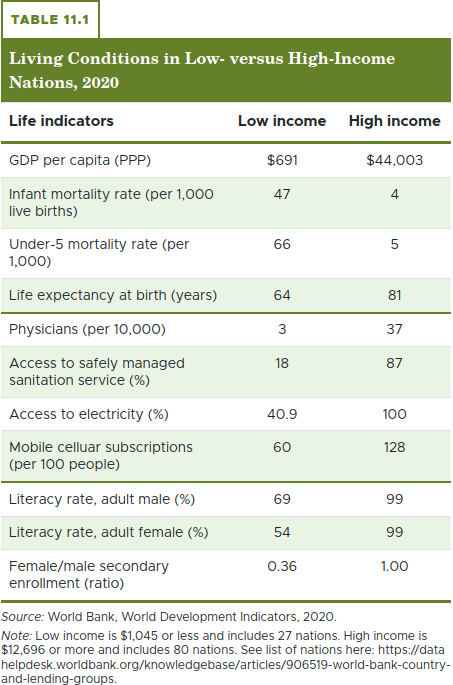
\includegraphics[scale=0.35]{../../images/Chapter 11/table 11.1.png}
\end{center}

The data in Table 11.1 support the contention that per capita GDP matters - not for the sake of more income per se, but because it correlates with better human welfare conditions, which matter to everyone.

\subsection*{Learning from the past}

We can learn a lot about the roots of economic growth by considering the past; historically, a common person's life focused on subsistence, simply trying to find enough food, shelter, and clothing to survive. As we saw in the previous section, even today many people still live on the margins of subsistence; what can history tell us about how high -income nations achieved economic development? This answer will help clairfy possible policy alternatives.

\subsubsection*{We were all poor once}
When you look around the globe today, you see rich nations and poor nations; you can probably name many rich nations: the United States, Japan, Taiwan, and the Western European nations, among others. You might also know the very poor nations: much of Africa, parts of Latin America, and significant parts of Asia; but the world was not always this way. If we consider the longer history of humankind, only recently did the incomes of common people rise above subsistence level.

The Industrial Revolution, during which many economies moved away from agriculture and toward manufacturing in the 1800s, is at the very center of the big increase in world income growth. Beginning with the Industrial Revolution, the rate of technical progress increased so rapidly, it was able to outpace population growth. The foundation for the Industrial Revolution was laid in the preceding decades, and these foundations included private property protection and several technologies innovations. We don't claim that the Industrial Revolution was idyllic for those who lived through it, but legal and other institutional innovations of that era paved the way for the unprecedented gains in human welfare that people have since experienced.
\begin{center}
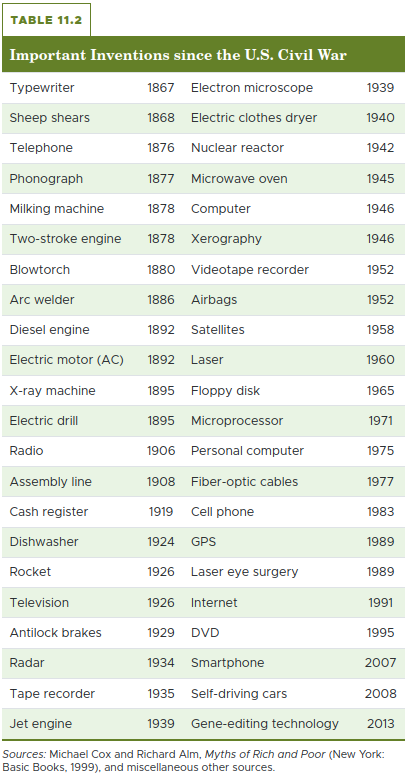
\includegraphics[scale=0.3]{../../images/Chapter 11/table 11.2.png}
\end{center}

This data do not imply that life is always easy and predictable comfortable for everyone in the modern world, but opportunities for the average person alive today are very different from those for the average person alive today are very different from those for the average person in past centuries. Table 11.2 lists a sampling of some of the major innovations of the past century and a half. Try to imagine life without any of these, and you'll get a sense of the gains we've made since the Industrial Revolution.

\subsubsection*{Some got rich, others stayed poor}

Although wealth has increased over the past two centuries, it is not evenly distributed around the globe. Figure 11.2 shows real per capita GDP (in 2020 U.S dollars) for various world regions. In 1820, the income of the average U.S citizen \$ 3,160, or about \$ 9 per day. Imagine trying to live  on \$ 9 per day in today's world - that is, \$ 9 to buy all the food, clothing, shelter, education, transportation, and anything else you might need to purchase. That was life in the United States in 1820, but it also describes the plight of many people in the world today.

\begin{center}
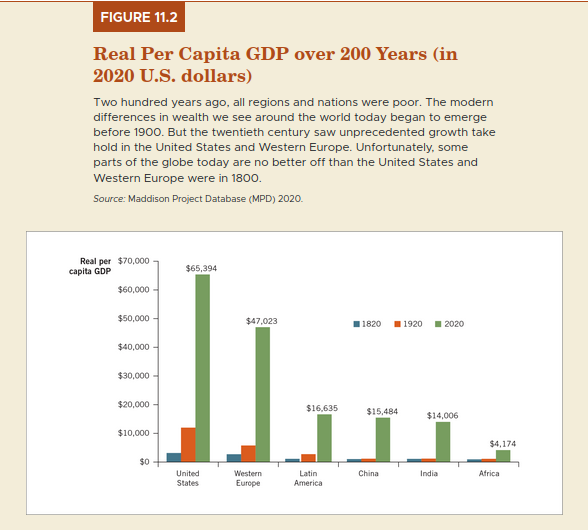
\includegraphics[scale=0.3]{../../images/Chapter 11/Figure 11.2.png}
\end{center}

While many of the current disparities between nations began about 200 years ago, some nations have moved from poor to rich as recently as the past few decades.

\subsection*{Measuring Economic Growth}

Overall, people today are much wealthier than they were 200 years ago; however, this prosperity did not occur overnight. Rather, income grew a little bit each year; there is a striking mathematical truth about growth: small difference in growth rates lead to large differences in wealth levels over time.  In this section, we explain how economic growth rates are computed, and we consider the level of growth a nation needs for its population to experience significant improvements in living standards.

\subsubsection*{The Mathematics of growth rates}

\begin{center}
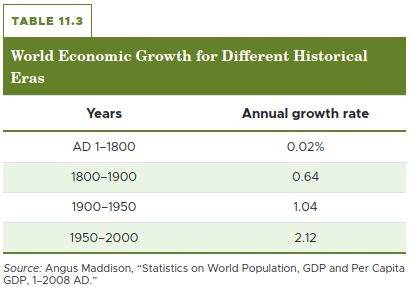
\includegraphics[scale=0.5]{../../images/Chapter 11/table 11.3 .png}
\end{center}

We have seen that economic growth is the annual growth rate of real per capita GDP. It is our measure of how an average person's income changes over time, including an allowance for price changes; but the government reports overall GDP data in nominal terms. Therefore, to get an accurate growth rate, we need to account for both inflation and population growth; we can use the following equation to approximate economic growth, where \(\% \Delta\) indicates the percentage change in a variable:
\begin{equation}
\text{economic growth} \approx \% \Delta \text{in nominal GDP}-\% \Delta \text{price level} - \% \Delta \text{population}
\end{equation}

A word of caution about terminology is in order. There's a big difference between nominal GDP growth, real GDP growth, and real per capita GDP growth. (In Table 11.4, these terms appear in orange.); but sloppy economic reporting sometimes confuses the terms. You may read something like "the U.S economy grew by 2.3\% in 2019," which refers to real GDP growth and is not calculated on a per capita basis; it would be an even bigger mistake to claim that U.S economic growth in 2019 was 4.1\% , a number not adjusted for either population growth or inflation. Such confusing wording is a common mistake in reports on international economic growth statistics.

\begin{center}
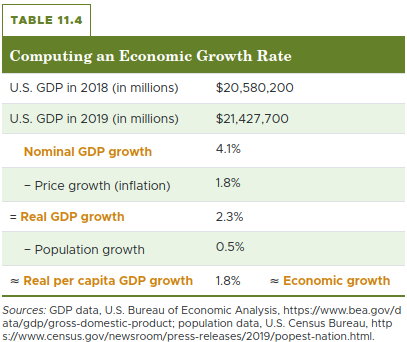
\includegraphics[scale=0.48]{../../images/Chapter 11/table 11.4 .png}
\end{center}

\subsubsection*{Growth rates and income levels}

Before we consider policies that might aid economic growth, we need to look more closely at how growth rates affect income level.

First, consider how significant it is when income doubles, or increases by 100\%. If your income doubled today - all else being equal - you could afford twice as much of everything you are currently buying. Now imagine what would happen if income doubled for an entire country or even for all countries. In the United States, real per capita GDP doubled in the 40 years between 1980 and 2020. This means that the average person living in the United States now can afford twice as much food, clothing, transportation, education, and even government services as the average U.S resident in 1980; that's quite a difference.

But increasing real income by 100\% in a single year is not realistic; let's use an annual growth rate closer to reality - say, 2\%, which has historically been an average rate of economic growth for the United States. With 2\% annual growth, how long does it take to double your income?

Table 11.5 illustrates the process of compounding over time by showing the increase from year to year.

\begin{center}
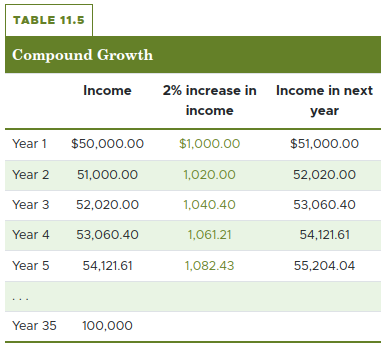
\includegraphics[scale=0.38]{../../images/Chapter 11/Table 11.5.png}\\
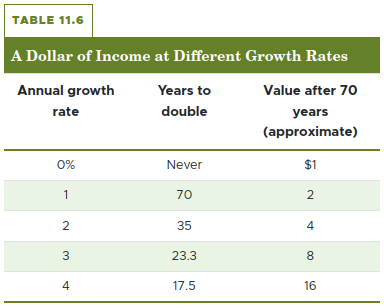
\includegraphics[scale=0.4]{../../images/Chapter 11/Table 11.6.png}
\end{center}

\subsubsection*{The Rule of 70}

We saw that when income grows at 2\% per year, it doubles in approximately 35 years. A simple rule known as the \textbf{rule of 70} determines the length of time necessary for a sum of money to double at a particular growth rate. According to the rule of 70: \textit{If the annual growth rate of a variable x\% , size of that variable doubles approximately every \(70 \div \text{x years}\).}

The rule of 70 is an approximation, but it works well with typical economic growth rates.

Table 11.6 illustrates the rule of 70 by showing how long it takes for a single dollar of income to double in value, given different growth rates.

The rule of 70 shows us that small and consistent growth rates, if sustained for a decade or two, can greatly improve living standards. Over the long course of history, growth rates were essentially zero, but the past two centuries have seen small, consistent growth rates, and the standard of living for many has increased dramatically.

We can look at actual growth rates of various countries over a long period to see the impact on income levels. Table 11.7 presents growth rates of several countries over the 66 years from 1950 to to 2016.

\begin{center}
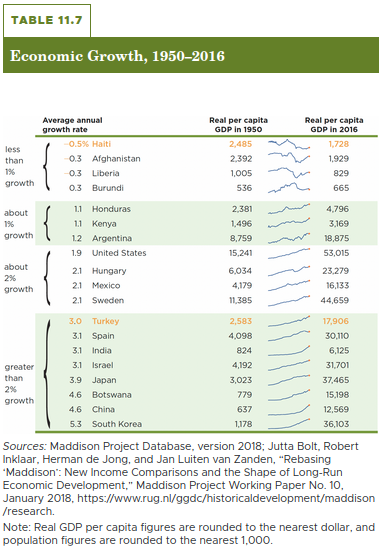
\includegraphics[scale=0.5]{../../images/Chapter 11/Table 11.7 .png}
\end{center}

Clearly, economic growth experiences have varied widely across time and place, but relatively small and consistent growth rates are sufficient to move a nation out of poverty the period of a few generation. And this movement out of poverty really matters for the people who live in these nations.
\begin{center}
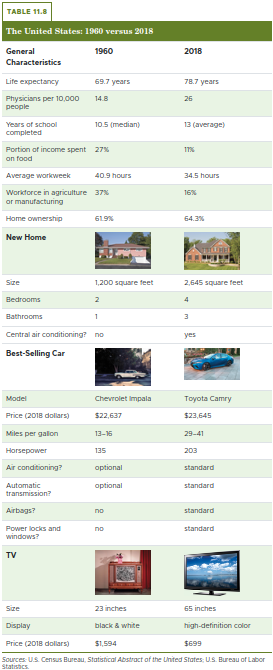
\includegraphics[scale=0.5]{../../images/Chapter 11/Table 11.8.png} \\ This correspond to the page above "%\newpage"
\end{center}

\newpage

\section*{How do resources and technology contribute to economic growth?}
At this point, you may wonder what can be done to provide the best opportunity for economic growth. We see economic growth in many, though certainly not all, nations; but even in those that have grown in the past, future growth is not assured. We now turn to major sources of economic growth.

Economists continue to debate the relative importance of the factors leading to economic growth. However, there is a general consensus on the significance of three factors for economic growth: \textit{resources, technology, and institutions}. In this section, we examine the first two; later in the chapter, we look at institutions.

\subsection*{Resources}
All else equal, the higher the quantity and quality of resources available, the more output a nation can produce. \textbf{Resources}, also known as \textbf{factors of production}, are the inputs used to produce goods and services. The discovery or cultivation of new resources is a source of economic growth; economists divide resources into three major categories: natural resources, physical capital, and human capital.

\subsubsection*{Natural Resources}
Natural resources include physical land and the inputs occurring naturally in or on the land. Coal, iron ore, diamonds, and lumber are examples of natural resources. Less obvious examples are mountains, beaches, temperate weather patterns, and scenic views - resources that residents enjoy consuming and that sometimes lead to tourism as a major industry.

Geography, or the physical location of a nation, is also a great resource that can contribute to economic growth. Geographical location facilitates trade and affect other important variables, such as weather and disease control; the world map in Figure 11.3 shows global GDP per square kilometer. As you can see, locations on coasts or along rivers have developed more rapidly than areas inland. These coastal or waterway-based locations were more naturally suited to trade in the days before railroads, trucks, and airplanes.

Natural resources clearly help to increase economic development, but they are not enough to make a nation wealthy; many poor nations are rich in natural resources.

\subsubsection*{Physical Capital}
The second category of resources is physical capital, or just capital. Recall that capital comprises the tools and equipment used in the production of goods and services. Examples of capital are factories, tractors, roads and bridges, computers, and shovels. \textbf{\textit{The purpose of capital is to aid in the production of future output}}.

\begin{center}
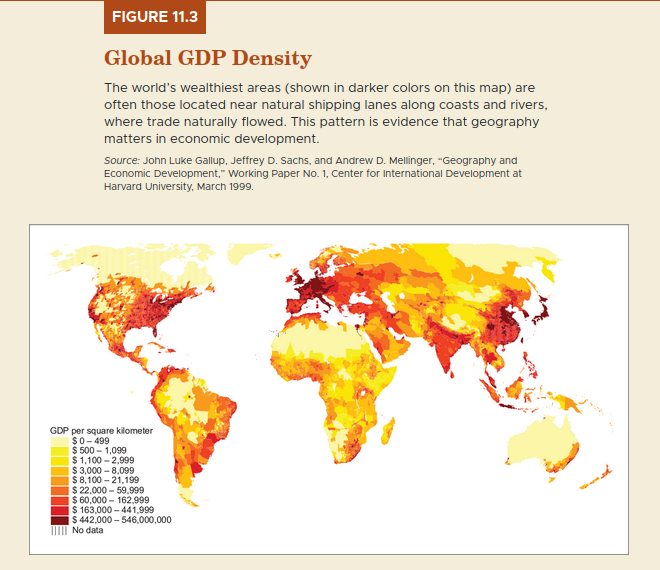
\includegraphics[scale=0.4]{../../images/Chapter 11/Figure 11.3 .png}
\end{center}

As the quantity of physical demand per worker rises, so does output per worker: workers are more productive with more and better tools. Look around the world: the productive nations have impressive roads, bridges, buildings, and factories; in poor nations, paved roads are nonexistent or in disrepair, vehicles are of lower quality, and computers are a luxury. Even public electricity and sewage treatment facilities are rare in parts of many developing nations.

Because of the obvious correlation between tools and wealth, many of the early contributions to growth theory focused on the role of physical capital. As a result, much international aid was used to build roads and factories, in the hope that prosperity would follow automatically; but today, most economists understand that capital alone is not sufficient to produce economic growth.

Factories, dams, and other larger capital projects bring wealth only when they mesh well with the rest of the economy. For example, a steel factory is of little use in a region better suited for growing corn; without a good rail network or proper roads, a steel factory cannot get the tools it needs and cannot easily sell it products. Damns fall into disrepair within a few years if they are not maintained. Water pipes are a wonderful modern invention, but if they are not kept in good shape, human waste from toilets contaminates the water supply...the point is that simply building new capital in a nation does not ensure future sustained economic growth.

\subsubsection*{Human Capital}
The output of a nation also depends on its workers. \textbf{Human capital} is the resource represented by the quantity, knowledge, and skills of the workers in an economy. It is possible to expand human capital by either increasing the number of workers available, educating the existing labor force, or both.

We often think in terms of the sheer quantity of workers: all else equal, a nation with more workers produces more output; but more output does not necessarily mean more economic growth. In fact, economic growth requires more output \textit{per capita}. Adding more workers to an economy may increase total GDP without increasing per capita GDP. However, if more worker from a given population enter the labor force, GDP per captia can increase.

There is another important dimension of human capital: the knowledge and skills of the workers themselves; in this context, it is possible to increase human capital through education and training. Training includes everything from basic literacy to college education and from software competencies to specific job training.

Not many people would doubt that a more educated labor force is more productive; and certainly, to boost per capita output, educating the labor force is more helpful than merely increasing the quantity of workers. But education alone is not enough to ensure economic progress.

\subsection*{Technology}

We know that the world would be much poorer without computers, automobiles, electric light bulbs, and other goods that have resulted from productive ideas. \textbf{Technology} is the knowledge available for the use in production; though technology is often embodied in machines and productive techniques, it is really just knowledge. New technology enables us to produce more while using fewer of our limited resources. A \textbf{technological advancement} introduces new techniques or methods so that firms can produce more valuable outputs per unit of input. We can either produce more with the same resources or use fewer resources to produce the same quantity.

Agriculture is a sector where technological advances are easy to spot. For example, we know that land resources are necessary to produce corn, but technological advances mean that over time it has become possible to grow and harvest more corn per acre of land. In fact, in the United States, the corn yield per acre is now six times what it was in 1930; we produce about 25 bushels of corn per acre, but now the yield is consistently over 150 bushels per acre. Higher yields are a result of technology that has produced hybrid seeds, herbicides, fertilizers, and irrigation techniques.

Like capital, technology produces value only when it is combined with other inputs. Simply carrying plans for a shoe factory to Haiti would not generate much economic value, the mere knowledge of how to produce shoes - while important - is only one piece of the growth puzzle. An economy must have the physical capital to produce shoes, must have the human capital to staff the factory and assembly line, and must create favorable conditions and incentives for potential investors. Economic growth occurs when all these conditions come together; that is one reason why it is incorrect to identify technological innovations as the sole cause of differences in wealth across nations.

Moreover, technological innovations do not occur randomly across the globe; some places produce large clusters of such innovations. Consider that information technology largely comes from MIT and Silicon Valley, movie and television ideas generally come from Hollywood, and new fashion designs regularly come from Paris, Milan, Tokyo, and New York. Technological innovations tend to breed more information; this conclusion leads us to reword an earlier question: Why do some regions innovate (and grow) more than others? A large part of the answer lies in our next topic, institutions.

\section*{What institutions foster economic growth?}

An \textbf{institution} is a significant practice, relationship, or organization in a society; are the official and unofficial conditions that shape the environment in which decisions are made. When we think of institutions, we normally focus on laws, regulations, and the type of government in a nation; but other institutions, such as social mores and work habits, are also important.

Institutions are not always tangible, physical items we can look at or hold. There might be a physical representative of an institution, such as the U.S Constitution or the building where the Supreme Court meets, but the essence of an institution encompasses expectations and habitual practices. The rules and the mindset within the Supreme Court are what is important, not the building or the chairs.

In this section, we consider the significant institutions that effect the nation's production and income. These include private property rights, political instability and the rule of law, competitive and open markets, efficient taxes, and stable money and prices. Many of these are examined in detail elsewhere in this book, so we cover them only briefly here.

\subsection*{Private Property Rights}

The single greatest incentive for voluntary production is ownership of what you produce; the existence of \textbf{private property rights} means individuals can own property - including houses, land, and other resources - and when they use their property in production, they own the resulting output.

\subsection*{Political Stability and the Rule of Law}

Political instability is a disincentive for investment; after all, investment makes sense only if there is a fairly certain payoff at the end. In an environment of political instability, there is no incentive to invest in either human or physical capital because there is no predictable future payoff.

Consistent and trustworthy enforcement of a nation's laws is crucial for economic growth. Corruption is one of the most common and dangerous impediments to economic growth; when government officials steal, elicit bribes, or hand out favors to friends, incentives for private investment are reduced. If individuals from all walks of life cannot count on a fair system and the opportunity to earn returns in their investment in human or physical capital, investment declines; and this decline reduces future growth.

The World Justice Project collected data on the rule of law across the world. Figure 11.5 shows the nations broken down into four groups, based on income, with an average rule-of-law index for each. It is no surprise that nations scoring in the top group on this index are also the nations with the highest levels of per capita GDP. The most corrupt nations are also those with the lowest level of income.

\begin{center}
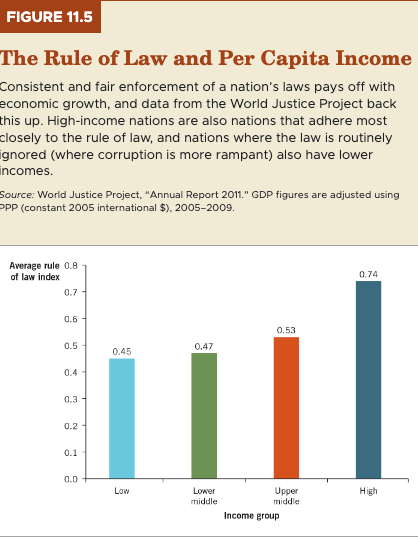
\includegraphics[scale=0.5]{../../images/Chapter 11/Figure 11.5.png}
\end{center}

\subsection*{Competitive and Open Markets}

In this section, we take a quick look at three institutions essential for economic growth: competitive markets, international trade, and the flow of funds across borders. These market characteristics are covered in detail elsewhere in this book.

\subsubsection*{Competitive Markets}
In \underline{Chapter 3}, we explored how competitive markets ensure consumers can buy goods at the lowest possible price. When markets aren't competitive, people who want to participate face barriers to entry, which inhibit competition and innovation; yet many nations monopolize key industries by preventing competition or by establishing government ownership of industries. These policies limit macroeconomic growth.

\subsubsection*{International Trade}
Recall from \underline{Chapter 2} that trade creates value; in some cases, trade enables nations to consume goods and services they would not produce on their own. Specialization and trade make all nations better off because each can produce goods for which it enjoys a comparative advantage. Output increases when nations (1) produce the goods and services for which they have the lowest opportunity cost and (2) trade for the other goods and services they wish to consume.

International trade barriers reduce the benefits available from specialization and trade. \underline{Chapter 19} is devoted to the study of international trade.

\subsubsection*{Flow of funds across borders}

In \underline{Chapter 9}, we talked about the importance of savings for economic growth. For example, the inflow of foreign savings has helped to keep interest rates low in the United States even as domestic savings rates have fallen. If firms and individuals are to invest in physical or human capital, someone has to save; opportunities for investment expand if there is access to savings from around the globe. That is, if foreigners can funnel their savings into your nation's economy, your nation's firms can use these funds to expand, however, many developing nations have restrictions on foreign ownership of land and physical capital within their borders. Restrictions on the flow of capital across borders handcuff domestic firms, which are then forced to seek funds solely from domestic savers.

\subsection*{Efficient taxes}

On the one hand, taxes must be high enough to support effective government; political instability, the rule of law, and the protection of private property rights all require strong and consistent government. And taxes provide the revenue to pay for government services, on the other hand, if we tax activities fundamental to economic growth, there will be fewer of these activities. In market economies, output and income are strictly intertwined; if we tax income, we are taxing output, and that is GDP. So although taxes are necessary, they can also reduce incentives for production.

Before the federal government instituted an income tax, government services were largely funded by taxes on imports; but international trade is also an essential institution for economic growth, so taxes on imports also impede growth.

\textit{Efficient taxes} are taxes sufficient to fund the activities of government while impeding production and consumption decisions as little as possible. It is not easy to determine the efficient level of taxes or even to determine what activities should be taxed. We will also discuss this issue further in Chapter 16, when we discuss fiscal policy.

\subsection*{Stable Money and Prices}

High and variable inflation is a sure way to reduce incentives for investment and production. In Chapter 9, we saw that inflation increases uncertainty about future price levels; when people are unsure about future price levels, they are more reluctant to sign contracts that deliver dollar payoffs in the future. Thus, unpredictable inflation diminishes future growth possibilities; in the United States, the Federal Reserve (the Fed) is charged with administering monetary policy. The Fed is designed to reduce incentives for politically motivated monetary policy, which typically leads to high variable inflation rates. We cover the Fed in greater detail in Chapter 17.

\section*{\textbf{How are some economists testing new ideas?}}

Measuring short-term impacts of growth is a challenge in economics; the 2019 Nobel Prize in Economics went to the development economists Abhijit Banerjee, Esther Duflo, and Michael Kremer for major contributions in this area. Duflo is the second female winner in economics and the youngest winner ever; the Nobel was given for pioneering fieldwork using randomized controlled trials (RCTs) in developing nations. An RCT randomly groups people to compare and test how policies and incentives affect economic growth.

For example, intestinal hookworms are common in developing countries and often keep students out of school. Using an RCT, Kremer found that deworming program had a much larger effect than anticipated; Kremer introduced deworming drugs into random school districts and saw improved health and less absenteeism. This included "spillover effects" to nearby communities, where deworming some individual reduced the chance that others would become infected; the program have since been expanded.

Using RCTs in India, Banerjee and Duflo found that plans involving "microcredit" - short-term business loans as small as \$ 20, given for no collateral - were not as helpful in reducing poverty as some had thought (though particularly enthusiastic entrepreneurs showed positive results). Duflo and Kremer also studied incentives given to farmers in developing countries to encourage investment in fertilizer for larger crop yields. They found it was most effective to offer discounts to purchase fertilizer at harvest time for future use.

Thus trio changed the practice of development economics. Economists now fan out around the globe testing new ideas in RCTs.

\section*{Conclusion}
In this chapter we considered the three sources of economic growth: resources, technology, and institutions; but we also cautioned against an overemphasis on resources and pointed to the necessity of growth-fostering institutions.

In the next chapter, we cover the theory of that supports this modern economic analysis.

\end{document}
